\documentclass{article}
\usepackage{graphicx} % Required for inserting images
\usepackage[T1]{fontenc}
\usepackage[croatian]{babel}
\usepackage{hyperref}
\usepackage{url}

\title{dzJakovCulo}
\author{Jakov Čulo}
\date{January 2024}

\begin{document}
\maketitle
\newpage
\tableofcontents
\newpage
\listoffigures
\newpage
\section{Zadatak}
IT i primjena\\
\begin{center}Domaća zadaća\end{center} 
\begin{center}Tekst zadatka\end{center} 
\begin{flushleft}Opći opis: student izrađuje popis komponenti za računalo željene namjene\end{flushleft} Potrebno je u LateXu izraditi detaljan opis konfiguracije osobnog računala. Dokument sadrži opis svake korištene komponente (npr. tvrdi disk Seagate, kapacitet 2TB, 7200RPM, 8MB cache, SATA3), fotografiju te obrazloženje zašto je korištena baš ta komponenta. Konfiguracija treba biti tehnički korektna, što podrazumijeva da bi računalo koje bi bilo sastavljeno prema odabiru komponenti bilo ispravno. Student treba obrazložiti svrhu računala i ciljanu uporabu “svog” računala prema odabiru komponenti (npr. CAD/CAM).\\ Konačno računalo treba imati i svu nužnu periferiju potrebnu za rad (monitor, tipkovnica…).\\\\ Dokument treba sadržavati pojedinačnu cijenu komponenti te ukupnu cijenu računala u EUR prema trenutnim tržišnim cijenama kao i izvor informacija o istima (referenca s poveznicom).\\\\ Korištene komponente trebaju biti aktualne (npr. CPU ne smije biti stariiji od 12. generacije Intela).\\\\ Student datoteke (.tex i .pdf ) učitava u GIT repozitorij (naziv repozitorija je Vaš JMBAG) kroz najmanje tri commita s odgovarajućom porukom.\\\\ Student u sustav Merlin učitava samo tektstualno datoteku koja sadrži poveznicu na repozitorij.
\newpage
\section{CPU}
AMD Ryzen 7 7800X3D
\begin{figure}[h]
    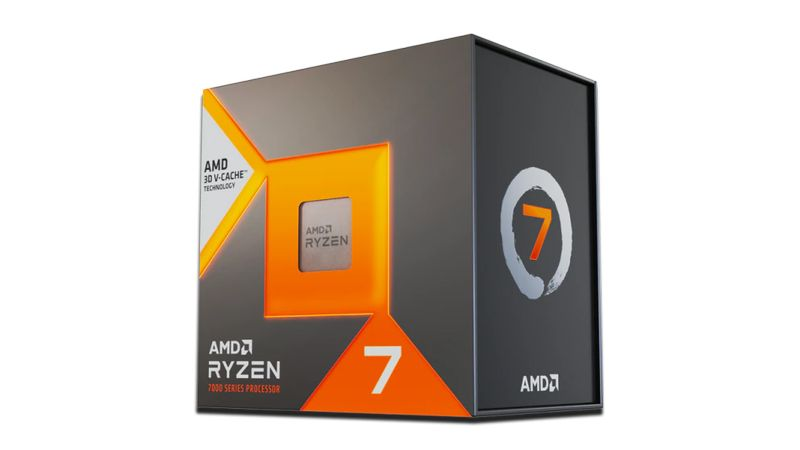
\includegraphics[width=12cm]{ryzen7800x3d.jpg}
    \caption{Ryzen 7 7800X3D}
\end{figure}\\
Socket: AM5\\
Broj jezgara: 8 \\
Niti: 16\\
Osnovna brzina: 4.2 GHz\\
Boostana brzina: 5 GHz\\
Cache memorija: 96 MB\\
120 W
Tehnologija: 5nm
Kompatibilnost: DDR5-SDRAM 3600,5200 MHz\\
Cijena: 477,89 €\\
\href{https://www.adm.hr/cpu-amd-ryzen-7-7800x3d-box-bez-coolera-420-500ghz-am5-100-100000910wof/77242/product/?utm_source=nabava.net&utm_campaign=nabava.net&utm_medium=click}{Link za CPU}
\newpage
\section{GPU}
Radeon RX 7900 XTX
\begin{figure}[h]
    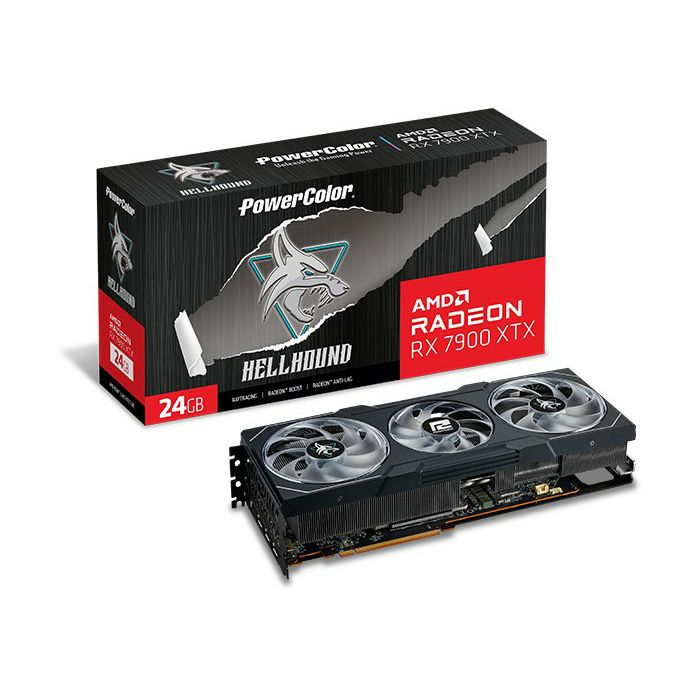
\includegraphics[width=10cm]{rx7900.jpg}
    \caption{Radeon RX 7900 XTX}
\end{figure}\\
Priključci: 1xHDMI 2.1, 3xDisplayPort 2.1\\
Memorija: 24GB GDDR6 , 2500MHz, 20Gbps 384bit, 960GB/s\\
Interface: PCIe 4.0 x16\\
Dimenzije: 320x118.5x62mm\\
Hlađenje: 3x axial fans (2x 100mm + 1x 90mm)\\
Vanjsko napajanje. 2x 8-pin PCIe\\
Tehnologija: TSMC 5nm + TSMC 6nm\\
Posebnosti: Real-time ray tracing, AMD Infinity Cache (96MB), HDCP 2.3, AMD FreeSync, AMD TrueAudio Next, AMD Eyefinity, AV1 Decode, 0dB zero-fan mode (up to 60°C), backplate, LED lighting (RGB), boost clock overclocked (+25MHz)  \\
Cijena: 1.209,47 €\\
\href{https://www.adm.hr/powercolor-rx7900xtx-hellhound-24gb-gddr6-rx-7900xtx-24g-loc/76343/product/}{Link za GPU}

\section{Matična ploča}
Asrock B650E PG-ITX WiFi, AM5, 90-MXBJE0-A0UAYZ
\begin{figure}[h]
    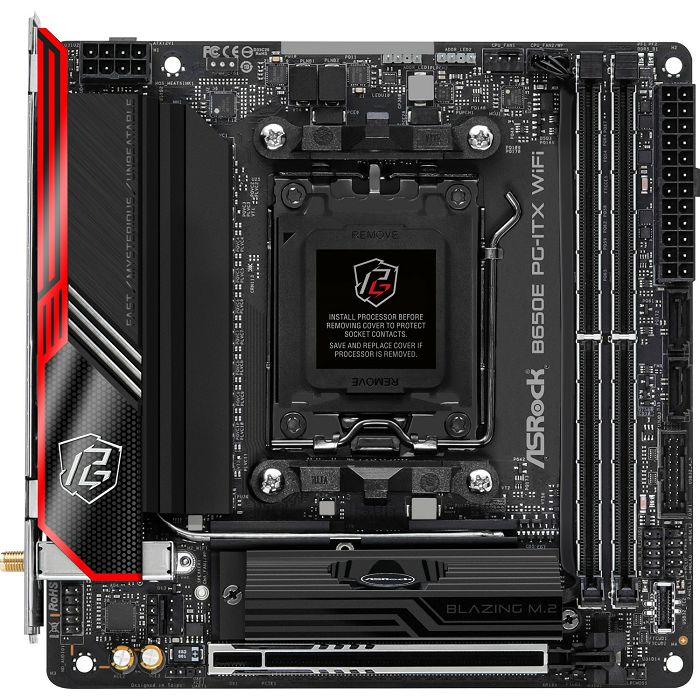
\includegraphics[width=12cm]{maticna.jpg}
    \caption{Asrock B650E PG-ITX}
\end{figure}\\
Socket:AMD AM5\\
Chipset:AMD B650E\\
CPU-Compatibility Ryzen 7000\\
RAM:2x DDR5 DIMM, dual PC5-51200U/DDR5-6400 (OC), max. 64GB (UDIMM)\\
Utori:1x PCIe 5.0 x16, 1x M.2/M-Key (PCIe 5.0 x4, 2280), 1x M.2/M-Key (PCIe 4.0 x4, 2280, back side), 1x M.2/E-Key (PCIe, 2230, occupied with WiFi+BT module), 1x HDMI 2.1 (iGPU), 1x USB-C 3.1 (10Gb/s), 3x USB-A 3.1 (10Gb/s), 4x USB-A 2.0 (480Mb/s), 1x 2.5GBase-T (Killer E3100G), 2x jack, 1x toslink, 2x antenna connector (RP-SMA), 1x USB-C 3.2 Key-A Header (20Gb/s), 1x USB 3.0 Header (5Gb/s, 2x USB 3.0), 1x USB 2.0 header (480Mb/s, 2x USB 2.0), 2x SATA 6Gb/s (B650E), 1x eDP-Header, 1x Speaker-Header\\
Header Cooling:1x CPU fan 4-Pin, 1x CPU fan/pump 4-Pin, 1x fan/pump 4-Pin\\
Wireless Wi-Fi 6E (WLAN 802.11a/b/g/n/ac/ax, 2x2), Bluetooth 5.2\\
RAID level 0/1/10 (B650E)\\
Power connections 1x 24-Pin ATX, 1x 8-Pin EPS12V\\
VRM 12 virtual phases (10+2), 12 real phases (10+2), PWM-Controller: RAA229620 (max. 12 phases)\\
Cijena: 363,16 € \\
\href{https://www.adm.hr/asrock-b650e-pg-itx-wifi-am5-90-mxbje0-a0uayz/76019/product/}{Link za Matičnu}
\newpage
\section{RAM}
DDR5 64GB (2x32) Corsair, 6000MHz, Vengeance RGB, CL30, AMD EXPO, CMH64GX5M2B6000Z30
\begin{figure}[h]
    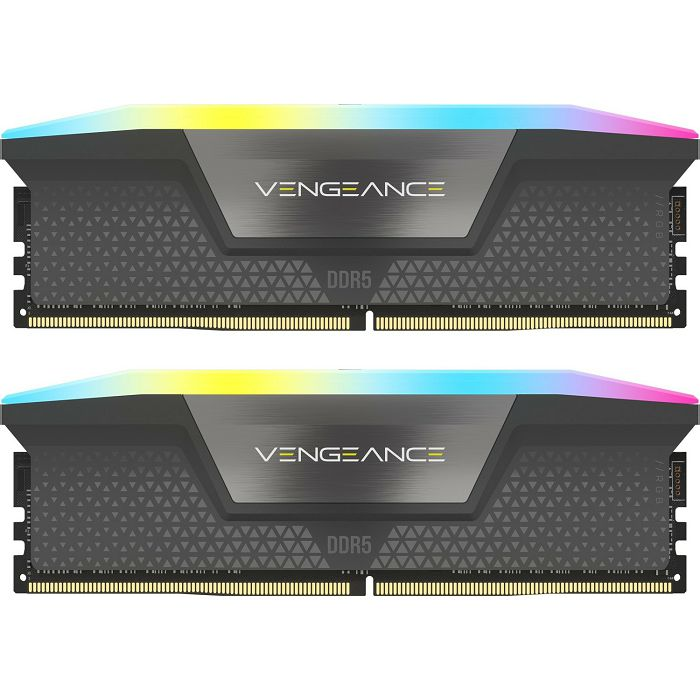
\includegraphics[width=10cm]{ram.jpg}
    \caption{ Corsair 6000MHz RAM}
\end{figure}\\
Tip: DDR5 DIMM 288-Pin, on-die ECC\\
Takt: 6000MHz\\
Moduli: 2x 32GB\\
Latencija: CAS Latency CL 30 (equivalent to ~10.00ns)\\
Osvjetljenje: Lighting RGB, Multi-Zone, 10 LED, Corsair iCUE, Gigabyte RGB Fusion, MSI Mystic Light Sync\\
Row-to-Column Delay tRCD 36 (equivalent to ~12.00ns)\\
Row Precharge Time tRP 36 (equivalent to ~12.00ns)\\
Active-to-Precharge Time tRAS 76 (equivalent to ~25.33ns)\\
Voltage 1.4V \\
Cijena: 336,84 € \\
\href{https://www.adm.hr/ddr5-64gb-2x32-corsair-6000mhz-vengeance-rgb-cl30-amd-expo-cmh6/78840/product/}{Link za RAM}
\newpage
\section{SSD}
Crucial SSD 2TB T700, M.2 SSD, NVMe PCIe, Gen 5, CT2000T700SSD5
\begin{figure}[h]
    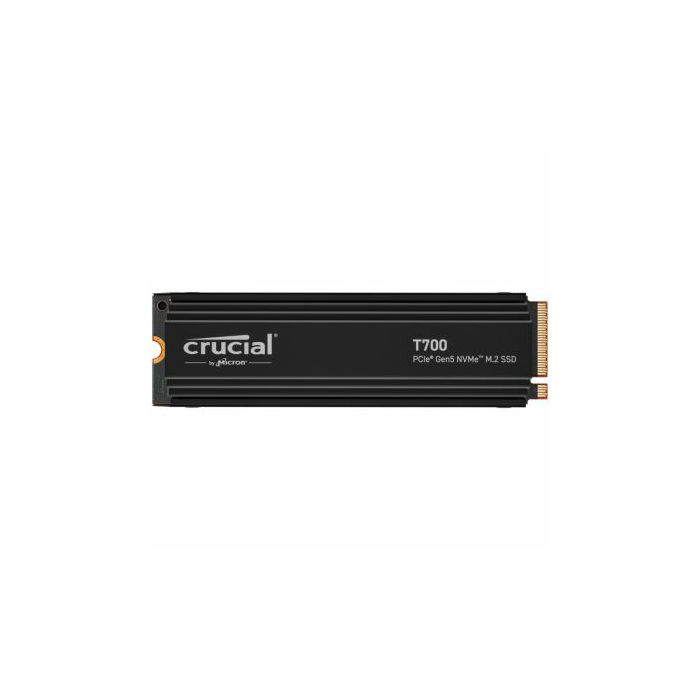
\includegraphics[width=10cm]{ssd.jpg}
    \caption{Crucial SSD 2TB}
\end{figure}\\
Tip: SSD\\
Interface: M.2/M-Key (PCIe 5.0 x4)\\
Čitanje: 12400MB/s\\
Pisanje: 11800MB/s SLC-Cached\\
Phison PS5026-E26, 8 channels cache\\
NVMe 2.0
Dimenzije: 80x23x21mm (with Cooling Blocks)\\
Veličina: 2TB\\
Posebnosti: M.2-Cooling Blocks\\
Cijena:415,79 €\\
\href{https://www.adm.hr/crucial-ssd-2tb-t700-m2-ssd-nvme-pcie-gen-5-ct2000t700ssd5/79439/product/}{Link za SSD}
\newpage
\section{Kučište}
Aerocool Midi Tower Cylon RGB ATX White, Window , ACCM-PV10012.21, 4713105950229
\begin{figure}[h]
    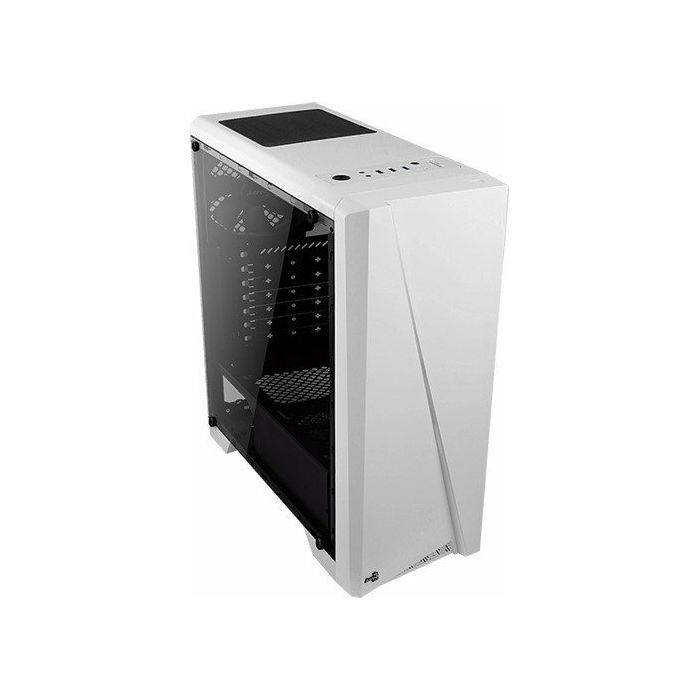
\includegraphics[width=10cm]{case.jpg}
    \caption{Aerocool Midi Tower Cyclon ATX}
\end{figure}\\
Utori: 2x 2.5"/3.5" (transverse, HDD rails), 3x 2.5"
front I/O 1x USB-A 3.0 (5Gb/s), 2x USB-A 2.0 (480Mb/s), 1x microphone, 1x headphone, 1x card reader (SD/SDHC/SDXC/microSD/microSDHC/microSDXC)
PCI-slots 7\\
Ventilatori:Fan(s) (front) 3x 120mm (optional), Fan(s) (rear) 1x 120mm, Fan(s) (top) 1x 120mm (optional), Fans (other) 2x 120mm (optional)\\
Kompatibilnost MBU: ATX\\
SVjetla: Lighting integrated RGB-LED lighting\\
Masa:3.80kg\\
Tip: Midi-Tower\\
Posebnosti:Cable Management, dust filter, acrylic window\\
Cijena: 62,11 €\\
\href{https://www.adm.hr/aerocool-cylon-rgb-atx-white-window-accm-pv1001221/72013/product/}{Link za Kučište}
\newpage
\section{PSU}
Napajanje Seasonic 850W G12 GC 850, 80 PLUS Gold, G12-GC-850
\begin{figure}[h]
    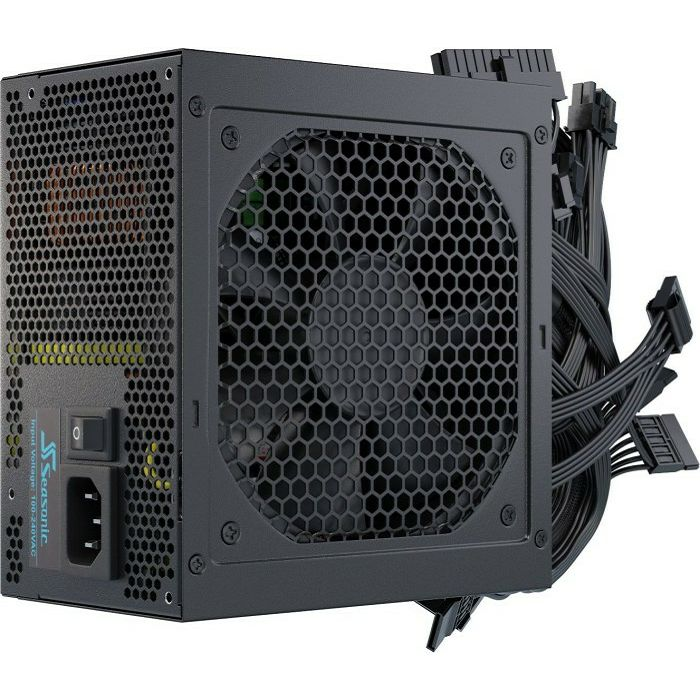
\includegraphics[width=10cm]{psu.jpg}
    \caption{Seasonic 850W}
\end{figure}\\
Snaga: 850W\\
Ventilator: 120mm\\
Konektori:1x 20/24-Pin, 2x 4/8-Pin ATX12V, 4x 6/8-Pin PCIe, 6x SATA, 3x IDE\\
Efikasnost: 90\% (Manufacturer), 89\% (80 PLUS, 115V)\\
Certifikat: 80 PLUS Gold (Manufacturer), 80 PLUS Gold (115V)\\
Dimenzije:150x86x140mm\\
Garancija: 5 godina\\
PFC active\\
shape factor ATX PS/2\\
Cijena:121,05 €\\
\href{https://www.adm.hr/napajanje-seasonic-core-g12-gc-850w-80-plus-gold-g12-gc-850/70724/product/}{Link za PSU}
\newpage
\section{Monitor}
DELL Alienware AW2724DM 27", Fast IPS, 2x DP, HDMI, USB, 180Hz, pivot
\begin{figure}[h]
    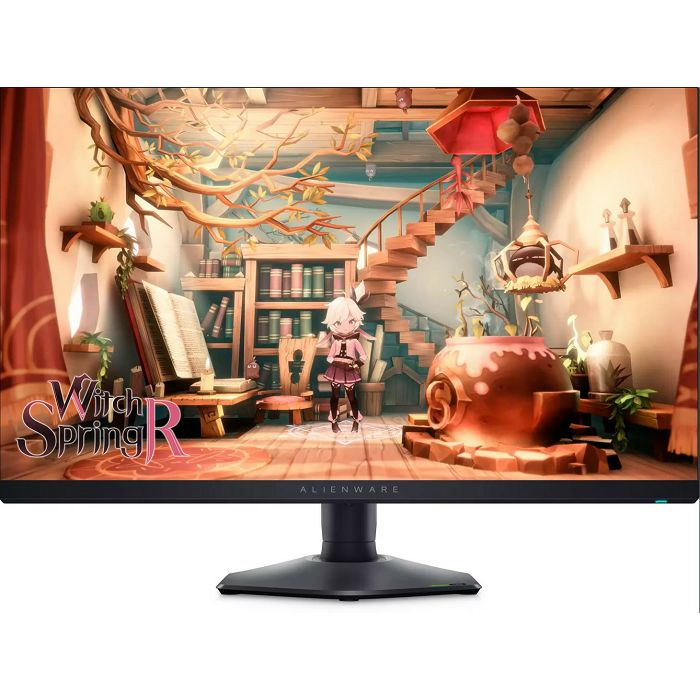
\includegraphics[width=10cm]{monitor.jpg}
    \caption{DELL Alienware monitor 27"}
\end{figure}\\
Tip ekrana: Fast IPS LED-backlit LCD 27", Anti-Glare with Low Blue Light technology\\
Omjer stranica:16:9\\
Rezolucija:  2560x1440 (DisplayPort (OC):180Hz, DisplayPort:165Hz, HDMI:144Hz);\\
Boje: 1.07 billion boja\\
Odaziv: 1ms\\
Maksimalni nagib: 178°/178°\\
Utori: 1x HDMI 2.1, 2x DisplayPort 1.4 (HDCP 1.4), 2x USB 3.2 Gen 1 downstream, 1x USB 3.2 Gen 1 upstream\\
Cijena: 484,21 €\\
\href{https://www.adm.hr/dell-alienware-aw2724dm-27-fast-ips-2x-dp-hdmi-usb-144hz-pivot/78256/product/}{Link za Monitor}
\newpage
\section{Slušalice}
Slušalice JBL Quantum 910X black/green, ANC, 2.4GHz wireless, bluetooth, JBLQ910XWLBLKGRN
\begin{figure}[h]
    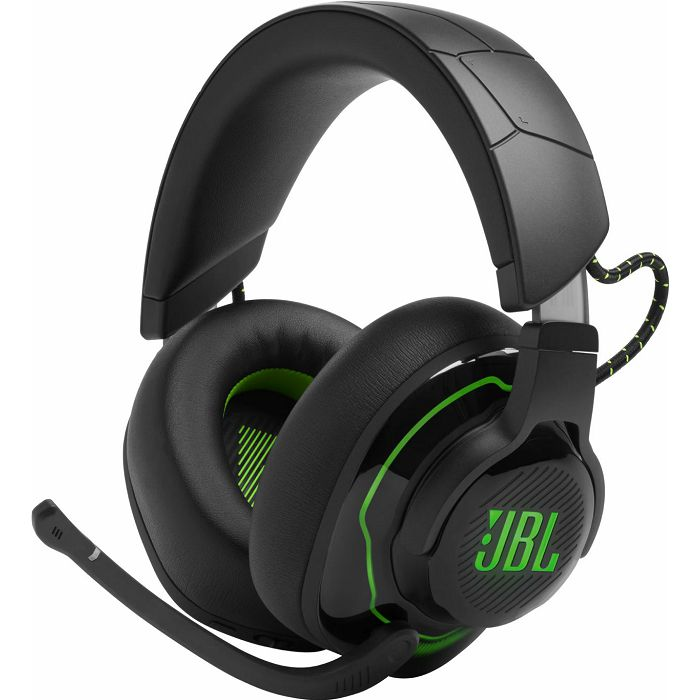
\includegraphics[width=10cm]{slusalice.jpg}
    \caption{Slušalice JBL Quantum 910X}
\end{figure}\\
Marka: JBL\\
Garancija: 2 godine\\
Audio channels 7.1\\
Sound reproduction Surround\\
Zvučni drivers 50 mm\\
Materijal: Plastika\\
Utor: USB port USB-C\\
Dizajn: zatvoren, spužva\\
Masa: 420 g\\
Boja: crno-zelena\\
Mikrofon: Ugrađen\\
Cijena: 294,74 €\\
\href{https://www.adm.hr/jbl-quantum-910p-white-blue-wireless-jblq910pwlwhtblu/76767/product/}{Link za Slušalice}
\newpage
\section{Tipkovnica}
Logitech Gaming G915 Lightspeed mehanička tipkovnica GL Clicky, USB/Bluetooth, 920-009111
\begin{figure}[h]
    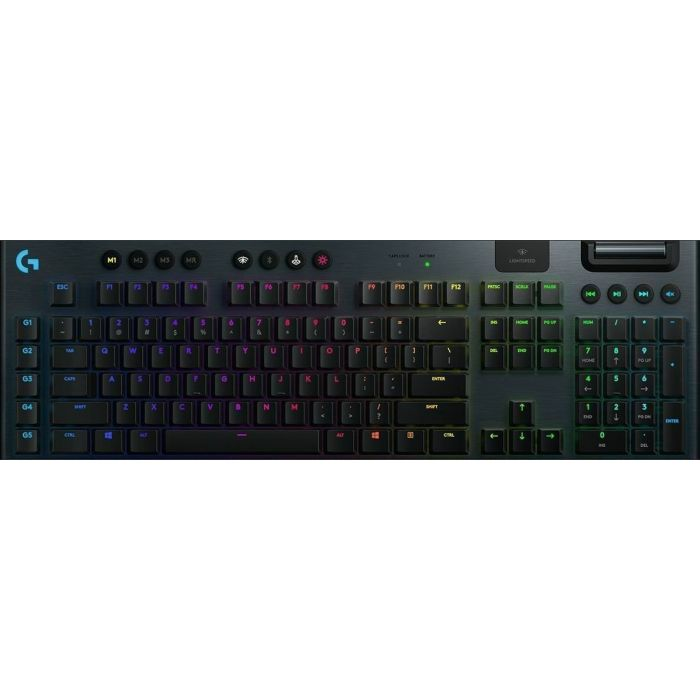
\includegraphics[width=10cm]{tipk.jpg}
    \caption{Logitech Gaming G915}
\end{figure}\\
Hod: 1,5mm\\
Marka: Logitech\\
Tip: mehanička, bežična\\
Potrebna snaga pritiska: 50g\\
2 profila osvjetljenja\\
3 profila makronaredbi\\
5 dodatnih G tipki\\
Napajanje trajanje baterije: do 30 sati\\
Masa: 1025g\\
Duljina PC kabela: 1,5m\\
Softver: DA\\
Cijena:283,16 €\\
\href{https://www.adm.hr/logitech-gaming-g915-lightspeed-mehanicka-tipkovnica-gl-clicky-usbbluetooth-920-009111/66469/product/}{Link za Tipkovnicu}
\newpage
\section{Miš}
Logitech G502 X plus RGB Lightspeed miš, black, 910-006162
\begin{figure}[h]
    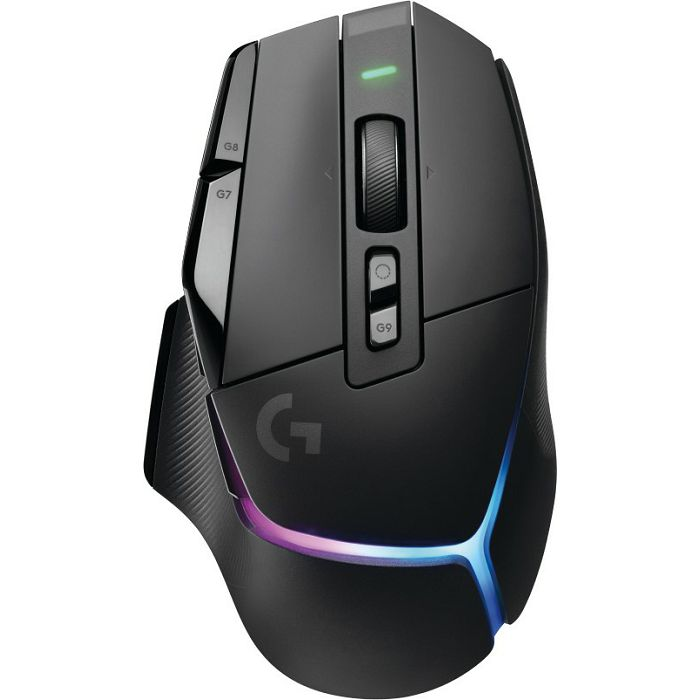
\includegraphics[width=10cm]{miš.jpg}
    \caption{Logitech G502 X plus}
\end{figure}\\
Za desnoruke\\
Tipke: 10 (entire), 2 (main), 4 (top), 3 (left), 1 (scroll wheel, 3 button functions)
resolution 25600dpi, reducible on 100dpi\\
sensor Logitech Hero 25K\\
sampling installment 1000Hz\\
Lighting Multi-colour (RGB)\\
Connection wireless (2.40GHz) or wired, USB\\
Napajanje: baterija (permanently installed), punjač (USB-C), \\
Dimenzije: (WxHxD) 79.2x41.1x131.4mm\\
Masa: 106g\\
Boja: crna\\
Softver: DA\\
Cijena: 178,95 €\\
\href{https://www.adm.hr/logitech-g502-x-plus-rgb-lightspeed-mis-black-910-006162/75978/product/}{Link za Miš}
\newpage
\section{Obrazloženje}
CPU-ovaj CPU je odabran jer je dovoljno jak i brz da podrži zahtjevne zadatke sa velikom kvalitetom\\
GPU-odabrana je zbog kompatibilnosti sa procesorom i zbog snažnih performansi\\
MBU-odabrana zbog kompatibilnosti \\
RAM-odabran zbog kompatibilnosti i radnog takta\\
SSD-odabran zebog brzine čitanja i pisanja te zbog veličine\\
Kučište-odabrano zbog kompatibilnosti te zbog izgleda\\
PSU-odabrano zbog snage te kompatibilnosti\\
Monitor-odabran zbog veličine, odaziva i refresha\\
Slušalice-odabrane zbog kvalitete\\
Tipkovnica-odabrana zbog brojnih dodatnih tipki i ljepoti\\
Miš-odabran zbog prilagodljivosti ruci, broju tipka, načina povezivanja\\
Korištenje:Igranje igara na visokoj rezoluciji, streaming, edit\\
Može obavljati bilo kakve zadatke normalnog čovjeka\\

Ukupna cijena: 4.227,37 €
\end{document}
